%!TEX root = ../Article.tex
% -- Author: Phil Steinhorst, p.st@wwu.de
\section{Kubische Komplexe}
	Wir beginnen mit einer Einführung des Begriffs des kubischen Komplexes. Dabei richten wir uns im Wesentlichen nach \cite{SchwerLectureNotes}.

\begin{defn}[Würfel, Seite]
	Eine \textbf{Seite} des $n$-Würfels $C=[0,1]^n \subseteq \RR^n, n \geq 1$, ist eine Teilmenge $F \subseteq C$ gegeben durch
	\[
		F = F_1 \times F_2 \times \dots \times F_n \text{ mit } F_i \in \{ \{0\}, \{1\}, [0,1]\}.
	\]
	Nach Definition ist auch $C$ eine Seite von $C$. Die auf $C$ eingeschränkte euklidische Metrik des $\RR^n$ bezeichnen wir mit $d_C$. Den $0$-Würfel definieren wir als $[0,1]^0 := \{0\}$. Wir nennen $\dim(C) := n$ die Dimension von $C$.
\end{defn}

\minisec{Bemerkung}
	Offensichtlich sind nichtleere Schnitte von Seiten eines $n$-Würfels $C$ wieder Seiten von $C$. Daher können wir Seiten der Kodimension $1$ von $C$ auch wie folgt definieren:
	\begin{equation}
	\begin{aligned}
		F_{i,e} :&= \{x \in C : x_i = e\} \text{ mit } e \in \{0,1\} \text{ und } i \in \{1, \dots n\} \\
		&= [0,1]^{i-1} \times \{e\} \times [0,1]^{n-i}
	\end{aligned}
	\end{equation}
	Seiten von höherer Kodimension sind dann nichtleere Schnitte von Seiten mit Kodimension $1$.
	
\begin{figure}[h]
\centering
\begin{tikzpicture}[scale=2]
	\draw [->,very thick] (0,0) -- (0,1.4) node[above] {$x_3$};
	\draw [->,very thick] (0,0) -- (1.4,0) node[right] {$x_1$};
	\draw [->,very thick] (0,0) -- (-.7,-.7) node[below] {$x_2$};

	\draw[schraffiert=orange] (-.5,-.5) -- (-.5,.5) -- (0,1) -- (0,0) -- (-.5,-.5);
	\draw [color=orange] (-.6,0) node[left] {$F_{1,0} = \{0\} \times [0,1]^2$};
	\draw[schraffiert=red] (.5,-.5) -- (.5, .5) -- (1,1) -- (1,0) -- (.5,-.5);
	\draw [color=red] (.7,-.4) node[right] {$F_{1,1} = \{1\} \times [0,1]^2$};
	\draw[schraffiert=blue] (-.5,.5) -- (.5,.5) -- (1,1) -- (0,1) -- (-.5,.5);
	\draw [color=blue] (.1,1.2) node[right] {$F_{3,1} = [0,1]^2 \times \{1\}$};
	\draw[ultra thick, color=teal] (.5,.5) -- (1,1);
	\draw (-.5,-.5) -- (.5,-.5);
	\draw [color=teal] (1.05,.9) node[right] {$F_{1,1} \cap F_{3,1} = \{1\} \times [0,1] \times \{1\}$};
\end{tikzpicture}
\caption*{Beispiele für Seiten eines $3$-Würfels}
\end{figure}

\begin{defn}[Klebung]
\label{klebung}
	Seien $C, C'$ zwei Würfel mit zugehörigen Seiten $F \subseteq C, F' \subseteq C'$. Eine bijektive Isometrie $\varphi\colon F \rightarrow F'$ heißt \textbf{Klebung} von $C$ und $C'$.
\end{defn}
\begin{figure}[h]
\centering
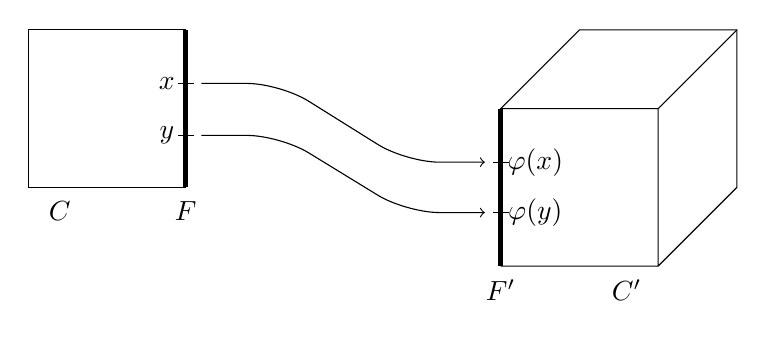
\begin{tikzpicture}[scale=2]
	\draw (1,0) -- (0,0) -- (0,1) -- (1,1);
	\draw [ultra thick] (1,0) -- (1,1);
	\draw (0.2,-.15) node {$C$};
	\draw (1,-.15) node {$F$};
	
	\draw (.95,0.33) -- (1.05,0.33) node[pos=-.7] {$y$};
	\draw (.95,0.66) -- (1.05,0.66) node[pos=-.7] {$x$};
	
	\draw (3,-.5) -- (4,-.5) -- (4,.5) -- (3,.5) -- (3.5,1) -- (4.5,1) -- (4.5,0) -- (4,-.5);
	\draw (4,.5) -- (4.5,1);
	\draw [ultra thick] (3,.5) -- (3,-.5);
	\draw (3,-.65) node {$F'$};
	\draw (3.8,-.65) node {$C'$};
	
	\draw (2.95,.16) -- (3.05,.16) node [pos=2.7] {$\varphi(x)$};
	\draw (2.95,-.16) -- (3.05,-.16) node [pos=2.7] {$\varphi(y)$};	
	
	\draw [->, rounded corners=12pt] (1.1,.66) -- (1.6,.66) -- (2.4,.16) -- (2.9,.16);
	\draw [->, rounded corners=12pt] (1.1,.33) -- (1.6,.33) -- (2.4,-.16) -- (2.9,-.16);
\end{tikzpicture}
	\caption*{Die Klebung $\varphi$ ist eine Isometrie, d.h. es gilt $d(x,y) = d'(\varphi(x),\varphi(y))$. \label{abb_klebung}}
\end{figure}

\begin{defn}[Kubischer Komplex]
\label{def:kub_kplx}
	Sei $\mathcal{C}$ eine Familie von Würfeln (i. A. verschiedener Dimensionen) und $\mathcal{S}$ eine Familie von Klebungen von Würfeln in $\mathcal{C}$ mit folgenden Eigenschaften:
	\begin{enumerate}[(i)]
		\item Kein Würfel ist mit sich selbst verklebt.
		\item Je zwei Würfel aus $\mathcal{C}$ sind höchstens einmal miteinander verklebt.
	\end{enumerate}
	\newpage
	Sei $\sim$ die durch
	\[
		x \sim y :\Leftrightarrow \text{ es existiert ein } \varphi \in \mathcal{S} \text{ mit } x \in \dom(\varphi) \text{ und } \varphi(x) = y
	\]
	erzeugte Äquivalenzrelation	auf der disjunkten Vereinigung $\sqcup_{C \in \mathcal{C}} C$. Dann definieren $\mathcal{C}$ und $\mathcal{S}$ den \textbf{kubischen Komplex} $X$ durch
	\[
		X := \enbrace*{\bigsqcup_{C \in \mathcal{C}} C} \diagup \sim.
	\]
\end{defn}
\begin{figure}[h]
\centering
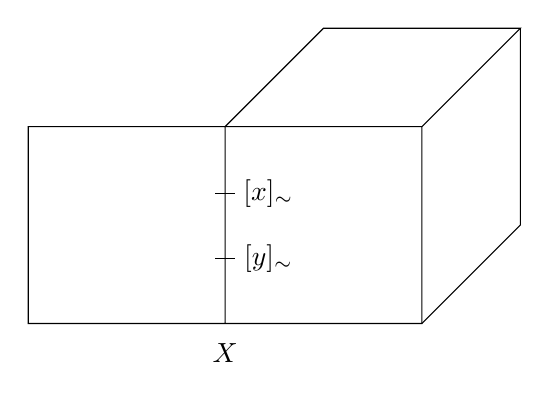
\begin{tikzpicture}[scale=2.5]
	\draw (2,1) -- (0,1) -- (0,0) -- (1,0) -- (1,1) -- (1.5,1.5) -- (2.5,1.5) -- (2,1) -- (2,0) -- (1,0);
	\draw (2,0) -- (2.5,.5) -- (2.5,1.5);
	\draw (1,-.15) node {$X$};
	\draw (.95,.33) -- (1.05,.33) node[pos=2.7] {$[y]_\sim$};
	\draw (.95,.66) -- (1.05,.66) node[pos=2.7] {$[x]_\sim$};
\end{tikzpicture}
	\caption*{Der kubische Komplex, der durch $\mathcal{C} = \{C,C'\}$ und $\mathcal{S} = \{\varphi\}$ aus der vorigen Grafik definiert wird.}
\end{figure}

Es folgen Beispiele für kubische Komplexe.
\begin{enumerate}[(1)]
	\item Bäume sind kubische Komplexe bestehend aus $0$- und $1$-Würfeln.
	\item $\RR^n$ lässt sich auf kanonische Weise mit Einheitswürfeln $C_i \simeq [0,1]^n$ überdecken ("kubulieren") und kann daher als kubischer Komplex aufgefasst werden.
	\item Der Torus ist ebenfalls als kubischer Komplex auffassbar.
\end{enumerate}
\begin{figure}[h]
\centering
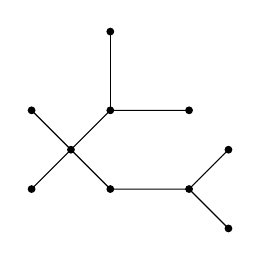
\begin{tikzpicture}[scale=1]
	\draw (0,0) -- (.5,.5) -- (1,0) -- (2,0) -- (2.5,-.5);
	\draw (2,0) -- (2.5,.5);
	\draw (0,1) -- (.5,.5) -- (1,1) -- (2,1);
	\draw (1,1) -- (1,2);
	\draw (0,0) node[fill,circle,inner sep=1pt]{};
	\draw (.5,.5) node[fill,circle,inner sep=1pt]{};
	\draw (0,1) node[fill,circle,inner sep=1pt]{};
	\draw (1,1) node[fill,circle,inner sep=1pt]{};
	\draw (1,2) node[fill,circle,inner sep=1pt]{};
	\draw (2,1) node[fill,circle,inner sep=1pt]{};
	\draw (1,0) node[fill,circle,inner sep=1pt]{};
	\draw (2,0) node[fill,circle,inner sep=1pt]{};
	\draw (2.5,-.5) node[fill,circle,inner sep=1pt]{};
	\draw (2.5,.5) node[fill,circle,inner sep=1pt]{};
\end{tikzpicture} \hspace{2cm}
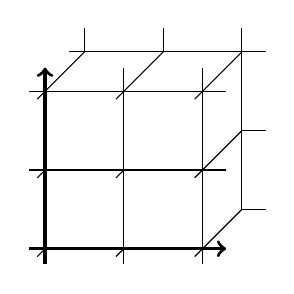
\begin{tikzpicture}[scale=1]
	\draw[->,very thick] (-.2,0) -- (2.3,0);
	\draw (-.2,1) -- (2.3,1); 
	\draw (-.2,2) -- (2.3,2); 
	\draw (.3,2.5) -- (2.8,2.5);
	
	\draw[->,very thick] (0,-.2) -- (0,2.3);
	\draw (1,-.2) -- (1,2.3);
	\draw (2,-.2) -- (2,2.3);
	\draw (2.5,.5) -- (2.5,2.8);
	
	\draw (-.1,1.9) -- (.5,2.5);
	\draw (.9,1.9) -- (1.5,2.5);
	\draw (1.9,1.9) -- (2.5,2.5);
	\draw (1.9,.9) -- (2.5,1.5);
	\draw (1.9,-.1) -- (2.5,.5);
	
	\draw (.5,2.5) -- (.5,2.8);
	\draw (1.5,2.5) -- (1.5,2.8);
	\draw (2.5,.5) -- (2.8,.5);
	\draw (2.5,1.5) -- (2.8,1.5);
	
	\draw (0,0) -- (-.1,-.1);
	\draw (1,0) -- (.9,-.1);
	\draw (0,1) -- (-.1,.9);
	\draw (1,1) -- (.9,.9);
\end{tikzpicture} \hspace{2cm}
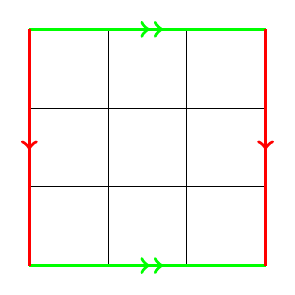
\begin{tikzpicture}[scale=1]
	\draw (0,1) -- (3,1);
	\draw (0,2) -- (3,2);
	\draw (1,0) -- (1,3);
	\draw (2,0) -- (2,3);
	
	\draw[color=green,very thick] (0,3) -- (3,3);
	\draw[->,color=green,very thick] (0,3) -- (1.7,3);
	\draw[->,color=green,very thick] (0,3) -- (1.53,3);
	\draw[color=green,very thick] (0,0) -- (3,0);
	\draw[->,color=green,very thick] (0,0) -- (1.7,0);
	\draw[->,color=green,very thick] (0,0) -- (1.53,0);
	
	\draw[color=red,very thick] (0,3) -- (0,0);
	\draw[->,color=red,very thick] (0,3) -- (0,1.47);
	\draw[color=red,very thick] (3,3) -- (3,0);
	\draw[->,color=red,very thick] (3,3) -- (3,1.47);
	\end{tikzpicture}
	\caption*{Beispiele für kubische Komplexe.}
\end{figure}

\begin{defn}[Weg, wegzusammenhängend]
	Sei $X$ ein kubischer Komplex. Ein \textbf{Weg} von $x \in X$ nach $y \in X$ ist eine Folge $\sigma = (x_0, \dots x_m)$ von Punkten $x_i \in X$ mit $x_0 = x$, $x_m = y$, sodass für alle $i$ mit $0 \leq i \leq m-1$ ein Würfel $C_i \in \mathcal{C}$ existiert mit $x_i, x_{i+1} \in C_i$. $X$ heißt \textbf{wegzusammenhängend}, falls für alle $x,y \in X$ ein Weg von $x$ nach $y$ existiert.
\end{defn}
\begin{figure}[h]
\centering
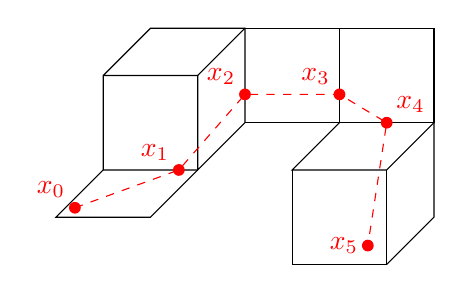
\begin{tikzpicture}[scale=1.2]
	\draw (1,0) -- (1,1) -- (0,1) -- (0,0) -- (1,0) -- (1.5,.5) -- (1.5,1.5) -- (.5,1.5) -- (0,1);
	\draw (1,1) -- (1.5,1.5);
	
	\draw (0,0) -- (-.5,-.5) -- (.5,-.5) -- (1,0);
	\draw (1.5,.5) -- (2.5,.5) -- (2.5,1.5) -- (1.5,1.5);
	\draw (2.5,1.5) -- (3.5,1.5) -- (3.5,.5) -- (2.5,.5);
	\draw (3.5,.5) -- (3,0) -- (2,0) -- (2.5,.5);
	\draw (2,0) -- (2,-1) -- (3,-1) -- (3,0);
	\draw (3,-1) -- (3.5,-.5) -- (3.5,.5);
	
	\draw [dashed, color=red] (-.3,-.4) node[fill,circle,inner sep=1.5pt]{} 
	-- (.8,0) node[fill,circle,inner sep=1.5pt]{} 
	-- (1.5,.8) node[fill,circle,inner sep=1.5pt]{} 
	-- (2.5,.8) node[fill,circle,inner sep=1.5pt]{} 
	-- (3,.5) node[fill,circle,inner sep=1.5pt]{} 
	-- (2.8,-.8) node[fill,circle,inner sep=1.5pt]{};
	
	\draw[color=red] (-.3,-.4) node[anchor = south east]{$x_0$};
	\draw[color=red] (.8,0) node[anchor = south east]{$x_1$};
	\draw[color=red] (1.5,.8) node[anchor = south east]{$x_2$};
	\draw[color=red] (2.5,.8) node[anchor = south east]{$x_3$};
	\draw[color=red] (3,.5) node[anchor = south west]{$x_4$};
	\draw[color=red] (2.8,-.8) node[anchor = east]{$x_5$};
\end{tikzpicture}
	\caption*{Die Punkte $x_1, \dots x_4$ des Weges $(x_0, \dots, x_5)$ liegen auf den "Klebestellen" der einzelnen Würfel.} 
\end{figure}
\newpage
Wir betrachten im folgenden, sofern nichts anderes gesagt wird, ausschließlich wegzusammenhängende kubische Komplexe. Sei $\sigma = (x_0, \dots, x_m)$ ein Weg von $x \in X$ nach $y \in X$. Da für alle $i$ die Punkte $x_i, x_{i+1}$ in einem $C_i \simeq [0,1]^{n_i} \subseteq \RR^{n_i}$ enthalten sind, können wir diesem Punktepaar den Abstand $d_{C_i} (x_i,x_{i+1})$ zuordnen. Die Summe
\[
	\ell(\sigma) := \sum\limits_{i=0}^{m-1} d_{C_i} (x_i,x_{i+1})
\]
bezeichnen wir als \textbf{Länge} des Weges $\sigma$. Dies ermöglicht uns, $X$ mit einer Metrik zu versehen:

\begin{lemma}[Längenmetrik]
	Sei $X$ ein wegzusammenhängender kubischer Komplex. Dann ist die Abbildung
	\begin{equation}
	\begin{aligned}
		d \colon X \times X &\longrightarrow \RR \\
		(x,y) &\longmapsto \inf\{ \ell(\sigma) : \sigma \text{ ist Weg von } x \text{ nach } y \text{ in } X\}
	\end{aligned}
	\end{equation}
	eine Metrik auf $X$ und heißt \textbf{Längenmetrik}. Wir nutzen daher die Bezeichnung kubischer Komplex auch für den metrischen Raum $(X,d)$.  
\end{lemma}

\minisec{Beweis}
	Symmetrie und $d(x,y) \geq 0$ ist klar, da die $d_{C_i}$ Metriken sind. Die Dreiecksungleichung folgt leicht aus der Tatsache, dass für zwei Wege $\sigma = (x, x_1, \dots, x_n, y)$ von $x$ nach $y$ und $\tau = (y, y_1, \dots, y_m, z)$ von $y$ nach $z$ ein Weg $\tau \circ \sigma := (x, x_1, \dots, x_n, y, y_1, \dots, y_m, z)$ von $x$ nach $z$ gegeben ist. Zur Definitheit:  Seien $x,y \in X$ beliebig. Ist $x = y$, dann existiert ein $C_i$ mit $x,y \in C_i$ und $\sigma = (x,y)$ ist ein Weg von $x$ nach $y$ mit $\ell(\sigma) = d_{C_i}(x,y) = 0$. Also ist $d(x,y) = 0$. Sei umgekehrt $d(x,y) = 0$ gegeben, dann existiert zu jedem $\varepsilon > 0$ ein Weg $\sigma_\varepsilon = (x_{\varepsilon,0}, \dots, x_{\varepsilon,n})$ von $x$ nach $y$ mit $\ell(\sigma_\varepsilon) < \varepsilon$. Dann ist aber auch $d_{C_{\varepsilon,i}}(x_{\varepsilon,i},x_{\varepsilon,i+1}) < \varepsilon$ für alle $0 \leq i \leq n-1$. Da $\varepsilon$ beliebig ist, folgt $d_{C_{\varepsilon,i}}(x_{\varepsilon,i},x_{\varepsilon,i+1}) \rightarrow 0$ und somit $x_{\varepsilon,i} \rightarrow x_{\varepsilon,i+1}$ für $\varepsilon \rightarrow 0$. Also ist $x = y$. \qed \\

Für einen kubischen Komplex $(X,d)$ betrachten wir das $1$-Skelett $X^{(1)}$, bestehend aus den Ecken und Kanten der einzelnen Würfel von $X$ (das heißt aus den Seiten der Dimension $0$ und $1$), sowie das $0$-Skelett $X^{(0)}$, welches aus den Eckpunkten der Würfel besteht. $X^{(1)}$ kann selbst als kubischer Komplex der Dimension $1$ aufgefasst werden.

\begin{defn}[simpliziale Metrik]
\label{def_D}
	Die Abbildung
	\begin{equation}
	\begin{aligned}
		D\colon  X^{(0)} \times X^{(0)} &\longrightarrow \RR \\
		(x,y) &\longmapsto \inf \{ \ell(\sigma) : \sigma \text{ ist Weg von } x \text{ nach } y \text{ in } X^{(1)}\}
	\end{aligned}
	\end{equation}
	heißt die \textbf{simpliziale Metrik} auf $X$.
\end{defn}

\minisec{Bemerkung}
	Die simpliziale Metrik ordnet zwei Eckpunkten $x$ und $y$ von $X$ die Länge des kürzesten Pfades zwischen $x$ und $y$ über die Kanten von $X$ zu. Offensichtlich ist $D$ eine Metrik, da $D$ mit der Längenmetrik auf dem kubischen Komplex $X^{(1)}$ (eingeschränkt auf $X^{(0)}$) übereinstimmt. Insbesondere gilt $d(x,y) \leq D(x,y)$ für alle $x,y \in X^{(0)}$, da jeder Weg in $X^{(1)}$ auch ein Weg in $X$ ist.

\begin{figure}[h]
\centering
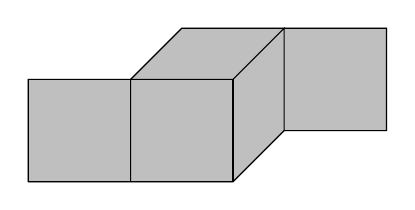
\begin{tikzpicture}[scale=1.3]
	\draw[fill,color=lightgray] (0,0) -- (1,0) -- (2,0) -- (2.5,0.5) -- (3.5,0.5) -- (3.5,1.5) -- (2.5,1.5) -- (1.5,1.5) -- (1,1) -- (0,1) -- (0,0);
	\draw (0,0) -- (1,0) -- (2,0) -- (2.5,0.5) -- (3.5,0.5) -- (3.5,1.5) -- (2.5,1.5) -- (1.5,1.5) -- (1,1) -- (0,1) -- (0,0);
	\draw (1,0) -- (1,1) -- (2,1) -- (2.5,1.5) -- (2.5,0.5);
	\draw (2,0) -- (2,1);
\end{tikzpicture} \hspace{2cm}
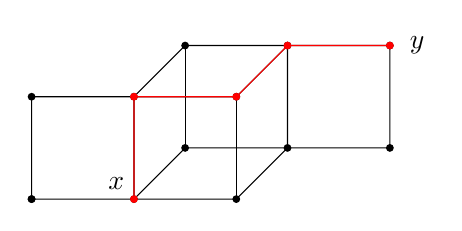
\begin{tikzpicture}[scale=1.3]
	\draw (0,0) node[fill,circle,inner sep=1pt]{} -- (1,0) node[fill,circle,inner sep=1pt]{} -- (2,0) node[fill,circle,inner sep=1pt]{} -- (2.5,0.5) node[fill,circle,inner sep=1pt]{} -- (3.5,0.5) node[fill,circle,inner sep=1pt]{} -- (3.5,1.5) node[fill,circle,inner sep=1pt]{} -- (2.5,1.5) node[fill,circle,inner sep=1pt]{} -- (1.5,1.5) node[fill,circle,inner sep=1pt]{} -- (1,1) node[fill,circle,inner sep=1pt]{} -- (0,1) node[fill,circle,inner sep=1pt]{} -- (0,0) node[fill,circle,inner sep=1pt]{};
	\draw (1,0) -- (1,1) -- (2,1) node[fill,circle,inner sep=1pt]{} -- (2.5,1.5) -- (2.5,0.5) -- (1.5,0.5) node[fill,circle,inner sep=1pt]{} -- (1,0);
	\draw (2,0) -- (2,1) ;
	\draw (1.5,0.5) -- (1.5,1.5);
	
	\draw[color=red] (1,0) node[fill,circle,inner sep=1pt]{} -- (1,1) node[fill,circle,inner sep=1pt]{} -- (2,1) node[fill,circle,inner sep=1pt]{} -- (2.5,1.5) node[fill,circle,inner sep=1pt]{} -- (3.5,1.5) node[fill,circle,inner sep=1pt]{};
	
	\draw (1,0) node[anchor=south east] {$x$};
	\draw (3.6,1.5) node[right] {$y$};
\end{tikzpicture}
	\caption*{Ein kubischer Komplex und sein $1$-Skelett. Es gilt $D(x,y) = 4$.} 
\end{figure}

Die nun folgenden Begriffe werden im nächsten Abschnitt hilfreich sein, um einen geschlossenen Ausdruck für die simpliziale Metrik zu finden.

\begin{defn}[Mittelwürfel]
	Der $i$-te \textbf{Mittelwürfel} von $C := [0,1]^n$ für $ \leq i \leq n$ ist gegeben durch
	\begin{equation}
	\begin{aligned}
		M_i :&= \penbrace*{x \in C : x_i = \frac{1}{2}} \\
		&= [0,1]^{i-1} \times \penbrace*{\frac{1}{2}} \times [0,1]^{n-i}
	\end{aligned}
	\end{equation}
\end{defn}

\begin{figure}[h]
\centering
\begin{tikzpicture}[scale=2]
	\draw [->,very thick] (0,0) -- (0,1.4) node[above] {$x_3$};
	\draw [->,very thick] (0,0) -- (1.4,0) node[right] {$x_1$};
	\draw [->,very thick] (0,0) -- (-.7,-.7) node[below] {$x_2$};
	
	\draw (-.5,-.5) -- (-.5,.5) -- (0,1) -- (0,0) -- (-.5,-.5);
	\draw (.5,-.5) -- (.5, .5) -- (1,1) -- (1,0) -- (.5,-.5);
	\draw (-.5,.5) -- (.5,.5) -- (1,1) -- (0,1) -- (-.5,.5);
	\draw (-.5,-.5) -- (.5,-.5);
	
	\draw [color=red,schraffiert=red] (-.25,-.25) -- (.75,-.25) -- (.75,.75) -- (-.25,.75) -- (-.25,-.25);
	\draw [color=teal,schraffiert=teal] (0,-.5) -- (.5,0) -- (.5,1) -- (0,.5) -- (0,-.5);
	\draw [color=blue,schraffiert=blue] (-.5,0) -- (.5,0) -- (1,.5) -- (0,.5) -- (-.5,0);
	
	\draw [color=teal] (0,-.5) node[below]{$M_1$};
	\draw [color=red] (-.4,.85) node{$M_2$};
	\draw [color=blue] (1.0,.5) node[right]{$M_3$};
\end{tikzpicture}
\caption*{Mittelwürfel eines $3$-Würfels}
\end{figure}

\begin{defn}[quadratäquivalent, transversal]
	Sei $X$ ein kubischer Komplex. Betrachte die durch
	\[ e \parallel e' \quad :\Leftrightarrow \quad e \text{ liegt gegenüber } e' \text{ in einem } 2\text{-Würfel von } X\]
	erzeugte Äquivalenzrelation auf der Menge der Kanten ($1$-Würfel) von $X$. Zwei Kanten $e, e'$ heißen \textbf{quadratäquivalent}, wenn $e \parallel e'$ gilt. \\
	Ein Mittelwürfel $M$ in $X$ heißt \textbf{transversal} zu $[e]_{\parallel}$ bzw. $e$, wenn $M \cap X^{(1)}$ aus Mittelpunkten von Kanten in $[e]_{\parallel}$ bzw. $e$ besteht. In diesem Fall schreiben wir $M \pitchfork [e]_{\parallel}$ bzw. $M \pitchfork e$.
\end{defn}

\begin{figure}[h]
\centering
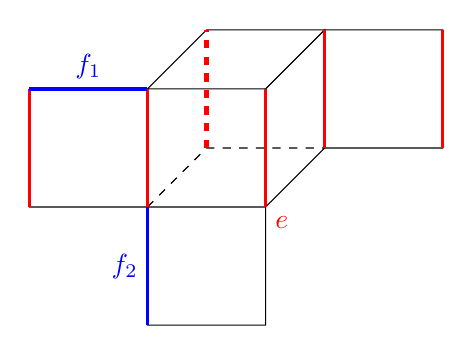
\begin{tikzpicture}[scale=1.5]
	\draw (2,2) -- (0,2) -- (0,1) -- (2,1) -- (2,0) -- (1,0) -- (1,2) -- (1.5,2.5) -- (3.5,2.5) -- (3.5,1.5) -- (2.5,1.5) -- (2,1) -- (2,2) -- (2.5,2.5) -- (2.5,1.5);
	\draw [dashed] (1,1) -- (1.5,1.5) -- (2.5,1.5);
	\draw [dashed,color=red,ultra thick] (1.5,1.5) -- (1.5,2.5);
	\draw [color=red, very thick] (2,1) -- (2,2);
	\draw [color=red, very thick] (1,1) -- (1,2);
	\draw [color=red, very thick] (0,1) -- (0,2);
	\draw [color=red, very thick] (2.5,1.5) -- (2.5,2.5);
	\draw [color=red, very thick] (3.5,1.5) -- (3.5,2.5);
	\draw [color=blue, very thick] (0,2) -- (1,2);
	\draw [color=blue, very thick] (1,0) -- (1,1);
	
	\draw [color=red] (2,1) node[anchor=north west]{$e$};
	\draw [color=blue] (.5,2) node[above] {$f_1$};
	\draw [color=blue] (1,.5) node[left] {$f_2$};
\end{tikzpicture}
\caption*{Rot markiert: Alle Kanten in $[e]_{\parallel}$. Die Kanten $f_1$ und $f_2$ sind nicht quadratäquivalent zu $e$.}
\end{figure}

\begin{defn}[Hyperebene, Halbräume]
	Sei $e$ eine Kante in einem kubischen Komplex $X$. Die Vereinigung $H(e)$ aller zu $[e]_{\parallel}$ transversalen Mittelwürfel heißt \textbf{Hyperebene} zu $e$.
	\[ H(e) := \bigcup_{M \pitchfork [e]_{\parallel}} M \]
	Eine Hyperebene $H$ in einem vollständigen $\cat$ kubischen Komplex $X$ partitioniert $X$ in die drei disjunkten Teilmengen $H, U^+$ und $U^-$, wie im Bild unten zu sehen ist (vgl. auch \cite{SchwerLectureNotes}, Prop. 3.4 und \cite{Sageev}, Prop. 4.10). $U^+$ und $U^-$ bezeichnen wir als \textbf{Halbräume} zu $H$.
\end{defn}

\begin{figure}[h]
\centering
\begin{tikzpicture}[scale=1.5]
	\draw (2,2) -- (0,2) -- (0,1) -- (2,1) -- (2,0) -- (1,0) -- (1,2) -- (1.5,2.5) -- (3.5,2.5) -- (3.5,1.5) -- (2.5,1.5) -- (2,1) -- (2,2) -- (2.5,2.5) -- (2.5,1.5);
	\draw [dashed] (1,1) -- (1.5,1.5) -- (2.5,1.5);
	\draw [dashed,color=red,ultra thick] (1.5,1.5) -- (1.5,2.5);
	\draw [color=red, very thick] (2,1) -- (2,2);
	\draw [color=red, very thick] (1,1) -- (1,2);
	\draw [color=red, very thick] (0,1) -- (0,2);
	\draw [color=red, very thick] (2.5,1.5) -- (2.5,2.5);
	\draw [color=red, very thick] (3.5,1.5) -- (3.5,2.5);
	\draw [color=red] (2,1) node[anchor=north west]{$e$};
	
	\draw [color=blue, very thick] (0,1.5) -- (1,1.5);
	\draw [color=blue, schraffiert=blue, very thick] (1,1.5) -- (2,1.5) -- (2.5,2) -- (1.5,2) -- (1,1.5);
	\draw [color=blue, very thick] (2.5,2) -- (3.5,2);
	
	\draw [color=blue] (.5,1.5) node[below] {$H_1$};
	\draw [color=blue] (1.5,1.5) node[below] {$H_2$};
	\draw [color=blue] (3,2) node[below] {$H_3$};
\end{tikzpicture} \hspace{2cm}
\begin{tikzpicture}[scale=1.5]
	\draw [color=teal,schraffiert = teal] (0,1.5) -- (0,2) -- (1,2) -- (1.5,2.5) -- (3.5,2.5) -- (3.5,2) -- (2.5,2) -- (2,1.5) -- (0,1.5);
	\draw [color=orange,schraffiert = orange] (0,1) -- (1,1) -- (1,0) -- (2,0) -- (2,1) -- (2.5,1.5) -- (3.5,1.5) -- (3.5,2) -- (2.5,2) -- (2,1.5) -- (0,1.5) -- (0,1);
	\draw [color=blue, ultra thick] (0,1.5) -- (2,1.5) -- (2.5,2) -- (3.5,2);
	
	\draw [thick] (2,2) -- (0,2) -- (0,1) -- (2,1) -- (2,0) -- (1,0) -- (1,2) -- (1.5,2.5) -- (3.5,2.5) -- (3.5,1.5) -- (2.5,1.5) -- (2,1) -- (2,2) -- (2.5,2.5) -- (2.5,1.5);
	
	\draw [color=teal] (0.5,2.05) node[above] {$U^+$};
	\draw [color=orange] (2.05,.5) node[right] {$U^-$};
	\draw [color=blue] (3.55,2) node[right] {$H(e)$};
\end{tikzpicture}
\caption*{Die Hyperebene zu $e$ ist gegeben durch $H(e) = H_1 \cup H_2 \cup H_3$. Es gilt $X = U^+ \cup H(e) \cup U^-$}
\end{figure}

Abschließend betrachten wir zwei bereits eingeführte Beispiele:
\begin{enumerate}[(1)]
	\item In einem Baum sind Mittelwürfel gerade die Mittelpunkte der Kanten. Da in einem Baum keine $2$-Würfel existieren, gibt es zu einer Kante $e$ keine weiteren quadratäquivalenten Kanten. Demzufolge ist der Mittelpunkt von $e$ die Hyperebene zu $e$.
	\item Im $\RR^n$ sind die Hyperebenen achsenparallele Ebenen der Kodimension $1$, also affine Untervektorräume der Form $H_{i,k} = \{(x_1,\dots,x_n) \in \RR^n : x_i = k - 0.5\}$ mit $1 \leq i \leq n$ und $k \in \ZZ$.
	\begin{figure}[h]
	\centering
		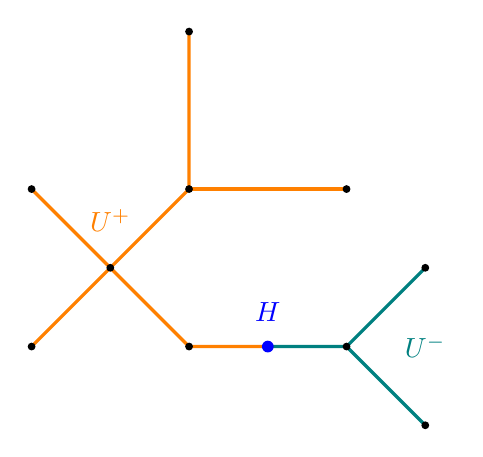
\begin{tikzpicture}[scale=2]
			\draw [very thick,color=orange] (0,0) -- (.5,.5) -- (1,0) -- (1.5,0);
			\draw [very thick,color=orange] (0,1) -- (.5,.5) -- (1,1) -- (1,2);
			\draw [very thick,color=orange] (1,1) -- (2,1);
			\draw [color=orange] (0.5,0.8) node{$U^+$};
			
			\draw [very thick,color=teal] (1.5,0) -- (2,0) -- (2.5,0.5);
			\draw [very thick,color=teal] (2,0) -- (2.5,-.5);
			\draw [color=teal] (2.5,0) node{$U^-$};
			
			\draw (0,0) node[fill,circle,inner sep=1pt]{};
			\draw (.5,.5) node[fill,circle,inner sep=1pt]{};
			\draw (0,1) node[fill,circle,inner sep=1pt]{};
			\draw (1,1) node[fill,circle,inner sep=1pt]{};
			\draw (1,2) node[fill,circle,inner sep=1pt]{};
			\draw (2,1) node[fill,circle,inner sep=1pt]{};
			\draw (1,0) node[fill,circle,inner sep=1pt]{};
			\draw (2,0) node[fill,circle,inner sep=1pt]{};
			\draw (2.5,-.5) node[fill,circle,inner sep=1pt]{};
			\draw (2.5,.5) node[fill,circle,inner sep=1pt]{};
			
			\draw [color=blue] (1.5,0) node[fill,circle,inner sep=1.5pt]{};
			\draw [color=blue] (1.5,0.1) node[above]{$H$};
		\end{tikzpicture} \hspace{2cm}
		\begin{tikzpicture}
			\path [schraffiert=teal] (-1.5,-1.5) rectangle (1.5,3.5);
			\path [schraffiert=orange] (1.5,3.5) rectangle (3.5,-1.5);
			
			\draw [color=teal] (-.5,-1.5) node[below]{$U^-$};
			\draw [color=orange] (3,-1.5) node[below]{$U^+$};
		
			\draw [->,ultra thick] (-1.5,0) -- (4,0) node[right]{$x_1$};
			\draw [->,ultra thick] (0,-1.5) -- (0,4) node[right]{$x_2$};
			\foreach \x in {-1,1,2,3} {
				\draw (-1.5,\x) -- (3.5,\x);
				\draw (\x,-1.5) -- (\x,3.5);
			}
			
			\foreach \x in {-1,0,...,3} {
				\draw [ultra thick, color=red] (1,\x) -- (2,\x);
			}
			
			\draw [color=red] (2,1) node[anchor=north west]{$e$};
			
			\draw [color=blue,ultra thick] (1.5,3.5) -- (1.5,-1.5) node[below] {$H_{1,2}$};
		\end{tikzpicture}
	\end{figure}
\end{enumerate}
	
\newpage